\documentclass[footexclude,twocolumn,DIV25,fontsize=10pt]{scrreprt} 

% Author: Siegfried Schöfer
% Comments, errors, suggestions: Siegfried.Schoefer@ce.stud.uni-erlangen.de

\usepackage[utf8]{inputenc}
\usepackage[T1]{fontenc}
\usepackage{textcomp}
\usepackage[english]{babel}
\usepackage{tabularx}
\usepackage{enumerate}
\usepackage{listings}
\usepackage{graphicx}
\usepackage{hyperref}

\setlength{\columnsep}{0.25em}
\makeatletter
\renewcommand{\section}{\@startsection{section}{1}{0mm}
	{-1.7ex}{0.7ex}{\normalfont\large\bfseries}}
\renewcommand{\subsection}{\@startsection{subsection}{2}{0mm}
	{-1.7ex}{0.5ex}{\normalfont\normalsize\bfseries}}
\makeatother
\setcounter{secnumdepth}{0}
\setlength{\parindent}{0em}
\pagestyle{empty}
\lstset{language=C++}

\begin{document}
\centerline{\Large{\textbf{OpenCL Cheat Sheet}}}
\centerline{based on OpenCL 1.1}
\section{Don't even try without}
\begin{lstlisting}[frame=tb]
#include <CL/cl.hpp>
\end{lstlisting}
Link to the OpenCL library (\textbf{-lOpenCL})
or let \textbf{CMake} do the job for you!
\subsection{Exception Handling}
\begin{lstlisting}[breaklines=true,frame=tb]
#define __CL_ENABLE_EXCEPTIONS

try {
  //...
} catch (cl::Error& err) {
  std::cerr<< "OpenCL: " << err.what() << "(" << err.err() << ")" << std::endl;
}
\end{lstlisting}

\section{Querying for devices}
\subsection{Get to know your platforms}
\begin{lstlisting}[breaklines=true,frame=tb]
std::vector<cl::Platform> platforms;
cl::Platform::get(&platforms);
\end{lstlisting}
\subsection{Get platform information}
\begin{lstlisting}[breaklines=true,frame=tb]
cl::Platform platform = platforms.front();
std::cout << platform.getInfo<CL_PLATFORM_NAME>() << std::endl;
\end{lstlisting}
\begin{tabularx}{\hsize}{lX}
  \verb*+CL_PLATFORM_PROFILE+ & embedded or full \\
  \verb*+CL_PLATFORM_VERSION+ & OpenCL version \\
  \verb*+CL_PLATFORM_EXTENSIONS+ & available extensions \\
  \verb*+CL_PLATFORM_NAME+ & i.e. Stream, CUDA \\
  \verb*+CL_PLATFORM_VENDOR+ & longer vendor info \\
\end{tabularx}
See OpenCL 1.1 Spec Chapter 4.1

\subsection{Get to know your devices}
\begin{lstlisting}[breaklines=true,frame=tb]
std::vector<cl::Device> devices;
platform.getDevices(CL_DEVICE_TYPE_DEFAULT, &devices);
\end{lstlisting}
\begin{tabularx}{\hsize}{lX}
  \verb*+CL_DEVICE_TYPE_CPU+ & \\
  \verb*+CL_DEVICE_TYPE_GPU+ & \\
  \verb*+CL_DEVICE_TYPE_ACCELERATOR+ & i.e. Cell \\
  \verb*+CL_DEVICE_TYPE_ALL+ & \\
\end{tabularx}

\subsection{Get device information}
\begin{lstlisting}[breaklines=true,frame=tb]
cl::Device device = devices.front();
std::cout << device.getInfo<CL_DEVICE_NAME>() << std::endl;
\end{lstlisting}
\begin{tabularx}{\hsize}{lX}
  \verb*+CL_DEVICE_MAX_COMPUTE_UNITS+ & \verb*+cl_uint+ \\
  \verb*+CL_DEVICE_MAX_WORK_ITEM_DIMENSIONS+ & \verb*+cl_uint+ \\
  \verb*+CL_DEVICE_MAX_WORK_ITEM_SIZES+ & \verb*+size_t[]+ \\
  \verb*+CL_DEVICE_MAX_WORK_GROUP_SIZE+ & \verb*+size_t+ \\
  \verb*+CL_DEVICE_MAX_CLOCK_FREQUENCY+ & \verb*+cl_uint+ \\
  \verb*+CL_DEVICE_MAX_MEM_ALLOC_SIZE+ & \verb*+cl_ulong+\\
  \verb*+CL_DEVICE_GLOBAL_MEM_SIZE+ & \verb*+cl_uint+\\
  \verb*+CL_DEVICE_GLOBAL_MEM_CACHE_SIZE+ & \verb*+cl_uint+\\
  \verb*+CL_DEVICE_GLOBAL_MEM_CACHELINE_SIZE+ & \verb*+cl_uint+ \\
  \verb*+CL_DEVICE_LOCAL_MEM_SIZE+ & \verb*+cl_uint+\\
\end{tabularx}
Much more on OpenCL 1.1 Spec. Chapter 4.2 ;-)

\section{Context}
A context is holding together buffers and compiled kernels.
\begin{lstlisting}[breaklines=true,frame=tb]
// select some devices in std::vector<cl::Device> devices
cl::Context context(devices);
\end{lstlisting}
Devices in the same context can share data (buffers).

\section{Command Queues}
For each device, you have to use your own command queue.
\begin{lstlisting}[breaklines=true,frame=tb]
// for each cl::Device you want to use
cl::CommandQueue cmdQueue(context, device);
\end{lstlisting}
Command are executed in-order automatically.
If you want to change that, you have to use:
\begin{lstlisting}[breaklines=true,frame=tb]
// for each cl::Device you want to use
cl::CommandQueue cmdQueue(context, device, CL_QUEUE_OUT_OF_ORDER_EXEC_MODE_ENABLE);
\end{lstlisting}
Events are helpful for synchronizing command queues which are organized out-of-order.
Otherwise you can enqueue a barrier.
\begin{lstlisting}[breaklines=true,frame=tb]
cmdQueue.enqueueBarrier();
\end{lstlisting}
You can have multiple command queues per devices.

\section{Buffers}
A buffer represents \textbf{global} memory on the device.\\
\subsection{Constructor}
\begin{lstlisting}[breaklines=true,frame=tb]
cl::Buffer(cl::Context& context, cl_mem_flags flags, size_t size, void *ptr = NULL) 
\end{lstlisting}
\begin{tabularx}{\hsize}{lX}
  \verb*+flags+ & \verb*+CL_MEM_READ_WRITE+\\ &\verb*+CL_MEM_READ_ONLY+\\ &\verb*+CL_MEM_WRITE_ONLY+ \\
  may be combined with & \verb*+CL_MEM_ALLOC_HOST_PTR+ \\
  & \verb*+CL_MEM_COPY_HOST_PTR+ \\
  & \verb*+CL_MEM_USE_HOST_PTR+ (\verb*+CL_MEM_COPY_HOST_PTR+ implied)\\
  \verb*+size+ & \verb*+sizeof(...)+ \\
  \verb*+ptr+ & pointing to the memory, that will be copied, only important when using \verb*+CL_MEM_COPY_HOST_PTR+ \\
\end{tabularx}
You can chain flags with \verb*+|+. If you use\verb*+CL_MEM_USE_HOST_PTR+, then \verb*+CL_MEM_COPY_HOST_PTR+ is implied.

\subsection{enqueueReadBuffer}
\begin{lstlisting}[breaklines=true,frame=tb]
cl::CommandQueue::enqueueReadBuffer(cl::Buffer& buffer, bool blocking, size_t offset, size_t size, void * ptr);
\end{lstlisting}
\begin{tabularx}{\hsize}{lX}
  \verb*+buffer+ & reference to your buffer \\
  \verb*+blocking+ & blocked write or unblocked write, effects ptr \\
  \verb*+ptr+ & pointing to the memory, that will be copied to the buffer \\
\end{tabularx}

\subsection{enqueueWriteBuffer}
\begin{lstlisting}[breaklines=true,frame=tb]
cl::CommandQueue::enqueueReadBuffer(cl::Buffer& buffer, bool blocking, size_t offset, size_t size, void * ptr);
\end{lstlisting}

\subsection{Mapped Pointers}
Instead of reading the buffer back to the host, then writing the buffer back again, you can just use a pointer to access the buffer’s memory.

\subsection{enqueueMapBuffer}
\begin{lstlisting}[breaklines=true,frame=tb]
void* cl::CommandQueue::enqueueMapBuffer(cl::Buffer& buffer, bool blocking, cl_map_flags flags, size_t offset, size_t size);
\end{lstlisting}
The pointer returned points to memory on the host and can be used in familiar ways.
\begin{tabularx}{\hsize}{lX}
  \verb*+flags+ & \verb*+CL_MAP_READ+ \\
  & \verb*+CL_MAP_WRITE+\\
\end{tabularx}
These flags can be combined. Open CL \textbf{Kernels} cannot access buffers with are flagged as \verb*+CL_MAP_WRITE+.

\subsection{enqueueUnmapMemObject}
Unmap the buffers, if you want to work on it with the kernels.
\begin{lstlisting}[breaklines=true,frame=tb]
void* cl::CommandQueue::enqueueUnmapMemObject(cl::Buffer& buffer, void* mapped_ptr);
\end{lstlisting}
\begin{tabularx}{\hsize}{lX}
  \verb*+mapped_ptr+ & pointer to the mapped memory got by enqueueMapBuffer \\
\end{tabularx}
Mapped pointers are an efficient way to access buffers if you use \verb*+CL_MEM_ALLOC_HOST_PTR+ when allocating them.
This then allows the use of pinned memory.

\subsection{enqueueCopyBuffer}
It's possible to copy a buffer to another buffer, without the host program getting involved. Nevertheless, the buffers have to be in the same context.
\begin{lstlisting}[breaklines=true,frame=tb]
cl::CommandQueue::enqueueCopyBuffer(cl::Buffer& src, cl::Buffer& dst, size_t src_offset, size_t dst_offset, size_t size);
\end{lstlisting}
If you want to ensure that \textbf{enqueueCopyBuffer} is finished you either have to use \textbf{Events} or cause the command queue to wait.
\begin{lstlisting}[breaklines=true,frame=tb]
// cmdQueue of type cl::CommandQueue
cmdQueue.finish();
\end{lstlisting}

\section{Events}
You can wait explicitly an event
\begin{lstlisting}[breaklines=true,frame=tb]
// event of type cl::Event
event.wait();
\end{lstlisting}

\subsection{enqueueReadBuffer}
\begin{lstlisting}[breaklines=true,frame=tb]
cl::CommandQueue::enqueueReadBuffer(cl::Buffer& buffer, bool blocking, size_t offset, size_t size, void * ptr, const std::vector<cl::Event> *events, cl::Event event);
\end{lstlisting}
\subsection{enqueueCopyBuffer}
\begin{lstlisting}[breaklines=true,frame=tb]
cl::CommandQueue::enqueueCopyBuffer(cl::Buffer& src, cl::Buffer& dst, size_t src_offset, size_t dst_offset, size_t size, const std::vector<cl::Event> *events, cl::Event event);
\end{lstlisting}
\begin{tabularx}{\hsize}{lX}
  \verb*+events+ & waiting for their completion \\
  \verb*+event+ & emits an event \\
\end{tabularx}

\section{Writing Kernels}
Example for an OpenCL kernel (further referred to by: vec.cl):
\begin{lstlisting}[breaklines=true,frame=tb]
__kernel void addVectors( __global float A, const __global float B, const __global float C, const unsigned int N) {
  int i = get_global_id (0);
  if (i<N) {
    A[i] = B[i] + C[i];
  }
}
\end{lstlisting}
\begin{itemize}
\item \verb*+__kernel+ has do be added to every function which is expected to be called from the \textit{host program}.
\item \verb*+get_global_id(x)+ is used for deciding which \textit{kernel} does what. In multi-dimensional problems $x \in \{0, 1, 2\}$.
\item \verb*+__global+ refers to the relatively big \textit{global} memory on the device.
\end{itemize}
If you want to use the double datatype, you have to paste the following code at the beginning of your kernel file. You also must have the extensions, the code activates.
\begin{lstlisting}[breaklines=true,frame=tb]
#if defined(cl_khr_fp64)  // Khronos extension available?
#pragma OPENCL EXTENSION cl_khr_fp64 : enable
#elif defined(cl_amd_fp64)  // AMD extension available?
#pragma OPENCL EXTENSION cl_amd_fp64 : enable
#endif
\end{lstlisting}
Other useful functions in a kernel:
\begin{lstlisting}[breaklines=true,frame=tb]
size_t indexSpaceX = get_global_size(x=0,1,2);
uint indexSpaceDim = get_work_dim()
\end{lstlisting}
\subsection{Address qualifiers}
\begin{itemize}
\item \verb*+__global+: global memory, everyone on the device can access it
\item \verb*+__local+: local memory, everyone in the same workgroup can access it
\item \verb*+__private+: registers of one single thread
\item \verb*+__constant+: constant memory
\end{itemize}

\section{Compiling an OpenCL kernel}
\begin{lstlisting}[breaklines=true,frame=tb]
// reading the source
ifstream input; string code;
input.open("./vec.cl", ifstream::in);
while (input.good()) {
  char c = input.get();
  code.append(1, c);
}
input.close();
// context is your OpenCL context
cl::Program::Sources source = cl::Program::Sources(1, std::make_pair(code.c_str(), code.size() - 1));
cl::Program program = cl::Program(context, source);
// devices is a std::vector<cl::Device> with the devices you want the kernel to run on
program.build(devices);
// you can get a build log for every device, here I used just the first device
std::cout << "Build Log: " << program.getBuildInfo<CL_PROGRAM_BUILD_LOG>(devices.front()) << std::endl;
cl::Kernel kernel = cl::Kernel(program, "addVectors");
\end{lstlisting}
Here you understand the importance of exceptions ;-).

\section{Executing the kernel}
It is easiest to use a kernel functor.
\begin{lstlisting}[breaklines=true,frame=tb]
// A, B, C are objects of cl::Buffer, N = 1024 represents the vector size
// cl::KernelFunctor cl::Kernel::bind(const CommandQueue &queue, const NDRange &global, const NDRange &local)
cl::KernelFunctor iAddVector = kernel.bind(cmdQueue, cl::NDRange(N), cl::NDRange(128));
// pass arguments directly to the functor
iAddVector(A, B, C, N);
\end{lstlisting}
In this example, N is expected to be a multiple of 128.
\textbf{local} determines the size of a workgroup.
OpenCL can choose the local workgroup size for you:
\begin{lstlisting}[breaklines=true,frame=tb]
cl::KernelFunctor iAddVector = kernel.bind(cmdQueue, cl::NullRange, cl::NullRange);
\end{lstlisting}
$\rightarrow$ No need for index checks!
But it may be chosen suboptimal as it influences how much local and private memory are available to the threads. 
You can create multi-dimensional index spaces by \verb*+cl::NDRange(x,y)+ or \verb*+cl::NDRange(x,y,z)+.

\section{Datatypes}
The native datatypes char, uchar, short, ushort, int, uint, long, ulong and float are availabe. In the host program you should add the prefix \verb*+cl_+ to the types. These prefixes can be dropped in the kernel.
OpenCL also supports vector datatypes with 2, 4, 8 and 16 elements. In OpenCL 1.1 support for 3 element vectors was added.
You get the vector datatype by adding the number of elements as a suffix to the datatype.
Of course you can define your own \verb*+struct+ with these basic types.

\section{Extensions}
This is only a small subset of all available extensions. There is a distinction between official extensions (\verb*+khr+) and vendor specific extensions.
\begin{itemize}
\item double precision floating point: \verb*+cl_khr_fp64+, \verb*+cl_amd_fp64+
\item half precision floating point: \verb*+cl_khr_fp16+
\item atomic functions: \verb*+cl_khr_global_int32_base_atomics+
\item Use multiple OpenCL platforms at once: \verb*+cl_khr_icd+
\end{itemize}

\section{Synchronization}
\subsection{Atomic functions}
This breaks the SIMD principle, so it probably also breaks your performance.
\subsection{Barriers}
You can use barriers in your kernels to synchronize accesses of workgroups to
\begin{itemize}
\item local memory: \verb*+barrier(CLK_LOCAL_MEM_FENCE);+
\item global memory: \verb*+barrier(CLK_GLOBAL_MEM_FENCE);+
\end{itemize}
\section{Restrictions}
Unfortunately, recursion cannot be used in OpenCL kernels.

\section{Optimization}
\begin{itemize}
\item latency hiding
\item coalescing
\item avoid synchronization
\item avoid branching in kernels
\end{itemize}

\begin{flushright}
\footnotesize
\rule{0.7\linewidth}{0.25pt}
\textbf{References}
\begin{itemize}
  \item Supercomputing on Graphics Cards - An Introduction to OpenCL and the C++ Bindings - Marcus Bannerman, Severin Strobl, Thorsten Pöschel \url{http://www.mss.cbi.uni-erlangen.de/?p1=lecturefeed&id=29&lang=} (visited 12.12.11)
  \item OpenCL page by Khronos, you will find all Specs there: \href{http://www.khronos.org/registry/cl/}{http://www.khronos.org/registry/cl/} (visited 12.12.11)
\end{itemize}
\rule{0.7\linewidth}{0.25pt}
\verb!Revision: 1.0, Date: !\today\\
\verb!Siegfried Schöfer (Siegfried.Schoefer@ce.stud.uni-erlangen.de)!
%
\includegraphics[totalheight=15mm]{logo_i3.png}

\includegraphics[totalheight=15mm]{fau.eps}
\includegraphics[totalheight=15mm]{by-sa.eps}
\\
This work is licensed under the Creative Commons Attribution-ShareAlike 3.0 Unported License. To view a copy of this license, visit \href{http://creativecommons.org/licenses/by-sa/3.0/}{http://creativecommons.org/licenses/by-sa/3.0/} or send a letter to Creative Commons, 444 Castro Street, Suite 900, Mountain View, California, 94041, USA.
\end{flushright}

\end{document}